%-------------------------------------------------------------------------------
%   圏論ノート
%   Keichi
%   圏論の勉強成果の個人的なまとめ
%-------------------------------------------------------------------------------

\documentclass{jsarticle}

\usepackage{listings,jlisting}
\usepackage[dvipdfm]{graphicx}
\usepackage{url}

%ソースコードの表示のデフォルトフォーマットを設定
\lstset{
    %言語
    language={Haskell},
    basicstyle={\small},
    %識別子のスタイル
    identifierstyle={\small},
    %コメントの書体
    commentstyle={\small\itshape},
    %キーワードの書体
    keywordstyle={\small\bfseries},
    ndkeywordstyle={\small},
    %文字列リテラルの書体
    stringstyle={\small\ttfamily},
    frame={htbp},
    %行が長くなったときの改行
    breaklines=true,
    columns=[l]{fullflexible},
    %行番号の表示
    %numbers=left,
    xrightmargin=0zw,
    xleftmargin=3zw,
    numberstyle={\scriptsize},
    stepnumber=1,
    numbersep=1zw,
    lineskip=-0.5ex
}


%-------------------------------------------------------------------------------
\begin{document}

\title{圏論ノート}
\author{Keichi}
\maketitle

\section{はじめに}
圏論を学ぶことはHaskellの型システムを理解する助けになりうる。
その対象がHaskellの型であり、射がHaskellの関数である、
「Haskell圏」というものを考えられる。\url{http://www.haskell.org/haskellwiki/Category_theory}

%-------------------------------------------------------------------------------
\section{圏}

\subsection{定義}
ある圏Cは、2つの集合の組からなる:

\begin{itemize}
    \item $Ob(C)$、$C$の「対象」の集合
    \item $Ar(C)$、$C$の「射」の集合
\end{itemize}

$Ar(C)$に含まれる射fは、$Ob(C)$の要素であるドメイン(もしくはソース)$dom f$と、
コドメイン(もしくはターゲット)$cod f$を持つ。$f:A \to B$と書けば、
fのドメインが$A$であり、コドメインが$B$であることを意味する。

\begin{figure}[htbp]
    \centering
    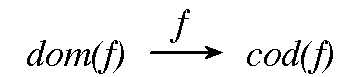
\includegraphics{diag_dom.pdf} 
\end{figure}

また合成という操作が存在し、これは$\circ$と表記される。
例えば、$g \circ f$において$f$のコドメインは$g$のドメインであり
、結局$g \circ f$のドメインとコドメインはそれぞれ$f$のドメインと$g$のコドメイン
となる。つまり、射$f$と$g$が存在し、$f:A \to B$かつ$g:B \to C$ならば、
$g \circ f = A \to C$ということである。また、ある対象$A$について、
$id_A: A \to A$という射が定義される。これは恒等射と呼ばれ、
$id$とだけ表記されることも多い。

\begin{figure}[htbp]
    \centering
    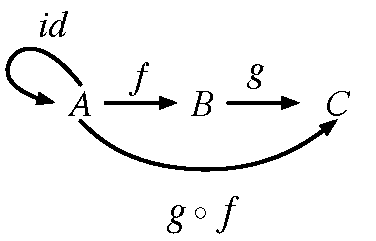
\includegraphics{diag_comp.pdf} 
\end{figure}

また、圏$C$においてHomset集合を
$hom_C(A,B)=\{f \mid f \in Ar(C), f: A \to B\}$と定義する

\subsection{公理}
また、$C$が圏であるためには、以下の条件が満たされている必要がある:
\begin{itemize}
    \item $f:A \to B$なら$f \circ id_A = id_b \circ f = f$
        (恒等射は左単位元、右単位元である)
    \item $f:A \to B$かつ$g: B \to C$か$h: B \to D$なら、
        $h \circ (g \circ f)=(h\circ g) \circ f$(射は結合律を満たす)
\end{itemize}

\subsection{圏の例}
\begin{itemize}
    \item Set, 集合を対象とし、集合間の写像を射とする
    \item Mon, モノイドを対象とし、モノイドの射を射とする
        (モノイドは対象が1つだけの圏ともとらえれる)
    \item Grp, 群を対象とし、群の準同型写像を射とする
    \item Hask, Haskellの型を対象とし、関数を射とする圏
    \item Cat, 圏を対象とし、関手を射とする圏の圏
    \item 関数を対象とし、データの流れを射とする圏(データフローダイアグラム)
\end{itemize}

\subsection{Haskellでの例}
Haskellの型と関数からなる圏Haskを考えると、
圏Haskの対象Ob(Hask)は全てのHaskellの型の集合、
\[\{Int, Bool, Float, String, \ldots\}\]
である。また、Ar(Hask)は全てのHaskellの関数の集合、
\[\{(+), length, even, \ldots\}\]
となる。圏Haskにおいて射の合成$\circ$は、
\begin{lstlisting}
    (.)::(b->c)->(a->b)->(a->c)
\end{lstlisting}
であり、恒等射は
\begin{lstlisting}
   id::a->a
\end{lstlisting}
となる。単位元律および結合律が成り立つのは明らかである。(seqなどの例外はあるが)

%-------------------------------------------------------------------------------
\newpage
\section{関手}

\subsection{定義}
$C$, $D$を圏とすると、関手$F:C \to D$は関数$F_{objects}:Ob(C) \to Ob(D)$
と関数$F_{arrows}:Ar(C)\to Ar(D)$の組である。前者は対象関数とよばれ、
後者は射関数とよばれる。

\begin{figure}[htbp]
    \centering
    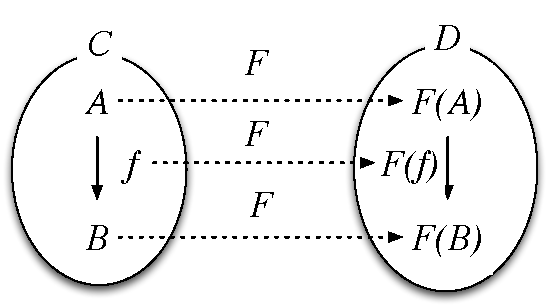
\includegraphics{diag_functor.pdf} 
\end{figure}

\subsection{公理}
\begin{itemize}
    \item 圏$C$において$f:A\to B$が存在すれば、
        圏$D$において$F(f):F(A)\to F(B)$
    \item 圏$C$において$g:B\to C$、$f:A\to B$が存在すれば、
        $F(f)\circ F(g)=F(f\circ g)$が成り立つ
    \item 圏$C$の全ての対象について、$id_{F(A)}=F(id_A)$:
\end{itemize}

\subsection{Haskellにおける関手}
厳密には、Haskell圏における関手は、Haskellの型と関数に対するあらゆる操作うち、
上記の公理を満たすものである。しかし、Haskellはプログラミング言語であるので、
実際Haskellで扱うのは、対象関数と射関数の両方がHaskellにおいて宣言でき、
名前をつけられる関手である。具体的には、Haskellにおける関手の対象関数は
多くの場合データコンストラクタであり、射関数は多相関数 fmapとなる。

\begin{lstlisting}
class Functor f where
    fmap :: (a -> b) -> (f a -> f b)
\end{lstlisting}

\subsection{Haskellによる例}
Haskellにおいて、ListやMaybe、Treeなどは全てFunctorクラスの
インスタンスであり、Functorクラスのインスタンスは以下の条件
\begin{lstlisting}
    fmap id = id
    fmap f . fmap g = fmap (f . g)
\end{lstlisting}
を満たすべきであるとされている。これは上記の公理に相当する。

具体的な例として、Hask圏からMaybe圏への関手Maybeを考える。
関手Maybeの対象関数はJustであり、射関数はfmapとなる。
\begin{lstlisting}
    --元の圏の上での関数f
    f :: Int -> Int
    f x =  x * x

    --fをMaybeの圏の射に写像する
    g :: Maybe Int -> Maybe Int
    g = fmap f

    --元の圏の上での値
    a = 2
    --aをMaybeの圏の対象に写像する
    b = Just a

    main = do
        --元の圏の上で対象に射を適用
        print $ f a
        --Maybeの圏の上で対象に射を適用
        print $ g b
\end{lstlisting}


%-------------------------------------------------------------------------------
\newpage

\section{自然変換}
\subsection{定義}
$C, D$を圏とし、$\Phi,\Psi:C\to D$を関手、$X,Y\in Ob(C)$とし、
$f\in hom_C(X,Y)$とする。

\begin{figure}[htbp]
    \centering
    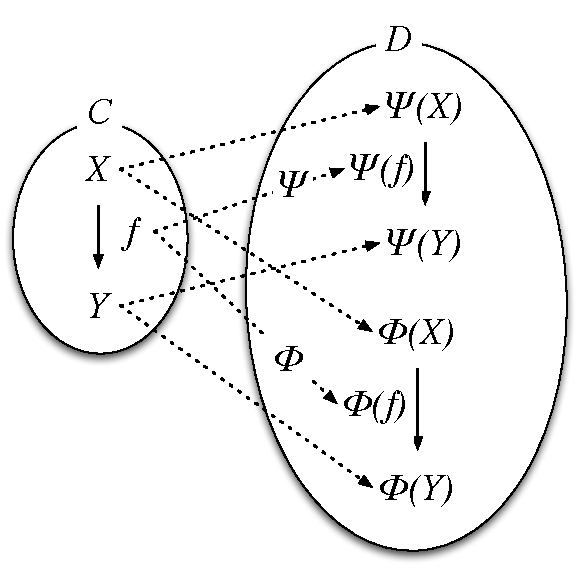
\includegraphics{diag_nt.pdf} 
\end{figure}

自然変換$\eta:\Phi\to\Psi$は、$C$の各対象を、
以下の条件を満たす$D$の射と対応づける。
\begin{itemize}
    \item $\forall A\in Ob(C)\to \eta_A\in hom_D(\Phi(A),\Psi(A))$
    \item $\eta_Y\circ \Phi(f)=\Psi(f)\circ\eta_X$
\end{itemize}
ここで、$\eta_A$を$A$における$\eta$のコンポーネントとよぶ。
よって、$D$において以下の図式が成り立つ。

\begin{figure}[htbp]
    \centering
    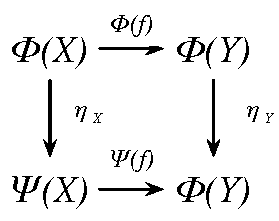
\includegraphics{diag_nt2.pdf} 
\end{figure}


\subsection{Haskellによる例}
\begin{lstlisting}
    maybeToList :: Maybe a -> [a]
    maybeToList Nothing     =   []
    maybeToList (Just a)    =   [a]

    main = do
        print $ fmap even $ maybeToList $ Just 5
        print $ maybeToList $ fmap even $ Just 5
\end{lstlisting}
この例と上の図式の対応関係を考えると、ファンクタ$\Psi$はList、
ファンクタ$\Phi$はMaybeとなる。自然変換$\eta_X$、$:\eta_Y$はmaybeToListに
相当する。(ここでmaybeToListは多相関数であるため、ηxとηyは
1つの関数maybeToListに集約される)また、$f$はevenであり
、これがfmapによってそれぞれ$\Psi(f)$と$\Phi(f)$にリフトされる。
fmapは多相であるため、$\Phi$、$\Psi$両方のファンクタの射部分に対応する。


\end{document}
